\documentclass{article}
\usepackage[utf8]{inputenc}
\usepackage{xcolor}
\usepackage{amsmath}
\usepackage{graphicx}
\usepackage{float}
\usepackage{minted}
\usepackage{circuitikz}
\usepackage{tikz}
\usetikzlibrary{shapes, arrows, calc, positioning, circuits.logic.US, circuits.logic.IEC}
\usepackage{geometry}
\geometry{a4paper, margin=1in}
\usepackage{hyperref}
\usemintedstyle{trac}

\usepackage{fancyhdr}
\pagestyle{fancy}
\fancyhf{}
\renewcommand{\headrulewidth}{0pt}
\fancyfoot[C]{\small 010153101 Digital Circuit and Microprocessor Fundamental}
\fancyfoot[R]{\thepage}

% Redefine plain style to match fancy style (for the title page)
\fancypagestyle{plain}{%
  \fancyhf{}%
  \fancyfoot[C]{\small 010153101 Digital Circuit and Microprocessor Fundamental}%
  \fancyfoot[R]{\thepage}%
  \renewcommand{\headrulewidth}{0pt}%
}

\title{Laboratory Exercise 4 \\ Decoders, Code Converters and Seven-Segment Displays}
\author{}
\date{}

\begin{document}

\maketitle

\section*{Introduction}
This laboratory exercise accompanies the first half of Lecture 5 (Combinational Circuit Building Blocks): the design procedure, decoders, encoders, code converters and the BCD (decimal) adder. All circuits are written in VHDL and tested on the DE0-CV board. You will learn how to use the \texttt{WITH SELECT} and \texttt{WHEN ... ELSE} statements to describe truth tables directly, how to combine small entities into larger ones, and how to display numbers on the seven-segment displays. The \texttt{hex7seg} decoder that you write in Part II will be reused in later labs (counters and microprocessors).

\section*{Objectives}
\begin{enumerate}
    \item To describe decoders and encoders in VHDL using selected and conditional signal assignments.
    \item To build a larger decoder from smaller decoders with enable inputs.
    \item To design a binary-to-seven-segment decoder and use it to display hexadecimal digits.
    \item To design a BCD (decimal) adder using binary adders and a correction circuit.
    \item To use the standard top-level entity template of the DE0-CV board.
\end{enumerate}

\section*{Equipment Required}
\begin{itemize}
    \item Intel DE0-CV board and a PC with Quartus Prime
    \item Files from Lab 3: \texttt{full\_adder.vhd} and \texttt{ripple\_adder\_4bit.vhd}
\end{itemize}

\section*{Pre-lab (complete before the session)}
The session is two hours long, so complete the following \emph{before} the session.
\begin{enumerate}
    \item Write the truth table of a $2$-to-$4$ decoder with active-high outputs and an enable input.
    \item Using Figure \ref{fig:seg}, fill in Table \ref{tab:seg} for the digits $0$ to $F$ (segment pattern with \textbf{1 = segment ON}). The DE0-CV displays are \textbf{active-low}: a segment is lit when its control signal is $0$. Two rows are given as examples.
\end{enumerate}

\begin{figure}[H]
    \centering
    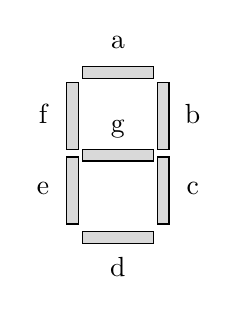
\begin{tikzpicture}[x=1cm,y=1cm]
        \tikzset{seg/.style={fill=gray!30, draw=black, thin}}
        \draw[seg] (0.25,2.1) rectangle (1.15,2.25); \node at (0.7,2.55) {a};
        \draw[seg] (1.2,1.2)  rectangle (1.35,2.05); \node at (1.65,1.65) {b};
        \draw[seg] (1.2,0.25) rectangle (1.35,1.1);  \node at (1.65,0.7) {c};
        \draw[seg] (0.25,0)   rectangle (1.15,0.15); \node at (0.7,-0.3) {d};
        \draw[seg] (0.05,0.25) rectangle (0.2,1.1);  \node at (-0.25,0.7) {e};
        \draw[seg] (0.05,1.2) rectangle (0.2,2.05);  \node at (-0.25,1.65) {f};
        \draw[seg] (0.25,1.05) rectangle (1.15,1.2); \node at (0.7,1.45) {g};
    \end{tikzpicture}
    \caption{Segments of a seven-segment display. On the DE0-CV board, \texttt{HEX0[0]} drives segment $a$, \texttt{HEX0[1]} drives $b$, \ldots, \texttt{HEX0[6]} drives $g$.}
    \label{fig:seg}
\end{figure}

\begin{table}[H]
    \centering
    \begin{tabular}{|c|c|c|c|c|c|c|c|}
        \hline
        \textbf{Digit} & $a$ & $b$ & $c$ & $d$ & $e$ & $f$ & $g$ \\
        \hline
        0 & 1 & 1 & 1 & 1 & 1 & 1 & 0 \\ \hline
        1 & 0 & 1 & 1 & 0 & 0 & 0 & 0 \\ \hline
        2 & & & & & & & \\ \hline
        3 & & & & & & & \\ \hline
        4 & & & & & & & \\ \hline
        5 & & & & & & & \\ \hline
        6 & & & & & & & \\ \hline
        7 & & & & & & & \\ \hline
        8 & & & & & & & \\ \hline
        9 & & & & & & & \\ \hline
        A & & & & & & & \\ \hline
        b & & & & & & & \\ \hline
        C & & & & & & & \\ \hline
        d & & & & & & & \\ \hline
        E & & & & & & & \\ \hline
        F & & & & & & & \\ \hline
    \end{tabular}
    \caption{Segment patterns (1 = segment ON).}
    \label{tab:seg}
\end{table}

\section*{Standard Top-Level Template}
From this lab on, the circuit that is downloaded to the board is described by a \textbf{top-level entity} whose ports are named like the board pins (\texttt{SW}, \texttt{KEY}, \texttt{LEDR}, \texttt{HEX0}, \ldots). The pin assignments can then be imported from the file supplied by your instructor (or from the DE0-CV User Manual) once, and reused in all later projects. The top-level entity simply connects the board pins to your own entities. Remember that \texttt{KEY} is active-low.

\begin{figure}[H]
    \centering
    \begin{minted}[frame=single, fontsize=\small, linenos]{vhdl}
LIBRARY ieee;
USE ieee.std_logic_1164.ALL;

ENTITY lab4_top IS
    PORT ( SW   : IN  STD_LOGIC_VECTOR(9 DOWNTO 0);
           KEY  : IN  STD_LOGIC_VECTOR(3 DOWNTO 0);
           LEDR : OUT STD_LOGIC_VECTOR(9 DOWNTO 0);
           HEX0 : OUT STD_LOGIC_VECTOR(6 DOWNTO 0);
           HEX1 : OUT STD_LOGIC_VECTOR(6 DOWNTO 0) );
END lab4_top;

ARCHITECTURE structural OF lab4_top IS
BEGIN
    -- instantiate your entities here and connect them to SW, KEY, LEDR, HEX
END structural;
    \end{minted}
    \caption{Top-level template for the DE0-CV board (add or remove ports as needed).}
    \label{fig:top}
\end{figure}

\section*{Part I: Decoders (about 25 min)}

A $2$-to-$4$ decoder with enable activates one of four outputs. With selected signal assignment, a truth table can be written directly in VHDL (Figure \ref{fig:dec_vhdl}). The operator \texttt{\&} joins signals into a longer vector (concatenation).

\begin{figure}[H]
    \centering
    \begin{minted}[frame=single, fontsize=\small, linenos]{vhdl}
LIBRARY ieee;
USE ieee.std_logic_1164.ALL;

ENTITY dec2to4 IS
    PORT ( A  : IN  STD_LOGIC_VECTOR(1 DOWNTO 0);
           EN : IN  STD_LOGIC;
           Y  : OUT STD_LOGIC_VECTOR(3 DOWNTO 0) );
END dec2to4;

ARCHITECTURE behavior OF dec2to4 IS
    SIGNAL sel : STD_LOGIC_VECTOR(2 DOWNTO 0);
BEGIN
    sel <= EN & A;
    WITH sel SELECT
        Y <= "0001" WHEN "100",
             "0010" WHEN "101",
             "0100" WHEN "110",
             "1000" WHEN "111",
             "0000" WHEN OTHERS;
END behavior;
    \end{minted}
    \caption{A 2-to-4 decoder with enable.}
    \label{fig:dec_vhdl}
\end{figure}

\begin{enumerate}
    \item Create a new Quartus project \texttt{lab4}, type the code of Figure \ref{fig:dec_vhdl} and simulate it for all combinations of $EN$ and $A$. Does the result agree with your pre-lab truth table?
    \item \textbf{3-to-8 decoder.} Write an entity \texttt{dec3to8} with inputs $A(2..0)$, $EN$ and output $Y(7..0)$ using two instances of \texttt{dec2to4}. The lower decoder is enabled when $EN=1$ and $A_2=0$; the upper decoder when $EN=1$ and $A_2=1$. Connect the outputs as $Y(3..0)$ and $Y(7..4)$. Draw the block diagram in your report.
    \item Simulate the 3-to-8 decoder for all 16 input combinations.
    \item Connect it to the board: $A$ = SW2--SW0, $EN$ = SW9 and $Y$ = LEDR7--LEDR0. Verify that only one LED is lit and that no LED is lit when $EN = 0$.
\end{enumerate}

\section*{Part II: Binary-to-Seven-Segment Decoder (about 30 min)}

The seven-segment decoder is used to display a 4-bit number on a HEX display. Its truth table (the entries of Table \ref{tab:seg}, but \textbf{inverted} because the displays are active-low) is written with a \texttt{WITH SELECT} statement. The segments are numbered \texttt{seg(0)} = $a$, \ldots, \texttt{seg(6)} = $g$, so the bit pattern is written as ``$gfedcba$''.

\begin{figure}[H]
    \centering
    \begin{minted}[frame=single, fontsize=\small, linenos]{vhdl}
LIBRARY ieee;
USE ieee.std_logic_1164.ALL;

ENTITY hex7seg IS
    PORT ( hex : IN  STD_LOGIC_VECTOR(3 DOWNTO 0);
           seg : OUT STD_LOGIC_VECTOR(6 DOWNTO 0) );   -- active low, seg(0)=a ... seg(6)=g
END hex7seg;

ARCHITECTURE behavior OF hex7seg IS
BEGIN
    WITH hex SELECT
        --          gfedcba
        seg <= "1000000" WHEN "0000",   -- 0
               "1111001" WHEN "0001",   -- 1
               -- TODO: complete the table for 2 ... F
               "1111111" WHEN OTHERS;   -- all segments off
END behavior;
    \end{minted}
    \caption{Skeleton of the hexadecimal seven-segment decoder.}
    \label{fig:hex7seg}
\end{figure}

\begin{enumerate}
    \item Complete the \texttt{hex7seg} entity using the patterns of Table \ref{tab:seg}. Remember to \textbf{invert} the patterns.
    \item Write a top-level entity using the template of Figure \ref{fig:top}: connect SW3--SW0 to \texttt{hex7seg} and the output to \texttt{HEX0}. Compile and download. Check that the display shows $0$ to $F$ correctly as you step through the switches.
    \item Extend the top-level so that SW7--SW4 are displayed on \texttt{HEX1}.
\end{enumerate}

\section*{Part III: Decimal (BCD) Adder (about 40 min)}

A BCD adder adds two decimal digits $A$ and $B$ (each $0$--$9$ coded in 4 bits) and produces a decimal result in the range $0$--$18$, displayed as two digits. As explained in Lecture 5, the 4-bit binary sum $Z = A + B$ must be corrected by adding $6$ ($0110_2$) whenever it exceeds $9$, and the carry then becomes the tens digit:
\[ K = C_{out} + Z_3 Z_2 + Z_3 Z_1 \]
where $C_{out}$ is the carry-out of the first adder, and the final result is $S = Z + 0KK0$, with $K$ also the tens digit.

\begin{figure}[H]
    \centering
    \begin{tikzpicture}[font=\small, node distance=1.2cm]
        \node[draw, minimum width=2.6cm, minimum height=1.4cm, align=center] (add1) at (0,0) {4-bit binary\\adder};
        \node[draw, minimum width=2.6cm, minimum height=1.4cm, align=center] (add2) at (5.5,0) {4-bit binary\\adder};
        \node[draw, minimum width=2.2cm, minimum height=1.0cm, align=center] (corr) at (2.75,-2.2) {correction\\logic $K$};
        \draw[->] (-3,0.4) node[left] {$A$} -- (add1.west |- 0,0.4);
        \draw[->] (-3,-0.4) node[left] {$B$} -- (add1.west |- 0,-0.4);
        \draw[->] (add1.east) -- node[above] {$Z$} (add2.west);
        \draw[->] (add1.east) ++(0.6,0) |- (corr.west);
        \draw[->] (add1.north) ++(0.8,0) -- ++(0,0.5) node[above] {$C_{out}$} ;
        \draw[->] (corr.east) -| (add2.south) node[pos=0.25, above] {$0KK0$};
        \draw[->] (add2.east) -- ++(1.4,0) node[right] {$S$ (units)};
        \draw[->] (corr.south) -- ++(0,-0.6) node[below] {$K$ (tens)};
    \end{tikzpicture}
    \caption{Block diagram of the BCD adder.}
    \label{fig:bcd}
\end{figure}

\begin{enumerate}
    \item Write an entity \texttt{bcd\_adder} that uses two instances of your \texttt{ripple\_adder\_4bit} from Lab 3 and the correction logic of the equation above. Hints: use \texttt{Cin => '0'} for both adders and \texttt{Cout => OPEN} for the unused carry output; the correction value is formed with the concatenation \texttt{"0" \& K \& K \& "0"}.
    \item Simulate the adder with $A+B$ equal to $0+0$, $4+5$, $9+1$, $9+9$ and $5+7$. Verify that the digits are correct.
    \item Make a top-level entity: $A$ = SW3--SW0, $B$ = SW7--SW4, the units digit on \texttt{HEX0} and the tens digit on \texttt{HEX1} (using \texttt{hex7seg}).
    \item Test the circuit on the board and record the results in Table \ref{tab:bcd} (the last row checks what happens with an invalid BCD digit).
\end{enumerate}

\begin{table}[H]
    \centering
    \begin{tabular}{|c|c|c|c|c|}
        \hline
        $A$ & $B$ & Tens (HEX1) & Units (HEX0) & Comment \\
        \hline
        0 & 0 & & & \\
        4 & 5 & & & \\
        9 & 1 & & & \\
        9 & 9 & & & \\
        7 & 8 & & & \\
        12 & 3 & & & \\
        \hline
    \end{tabular}
    \caption{BCD adder results on the board.}
    \label{tab:bcd}
\end{table}

\section*{Extension (take-home, or if time permits)}
\begin{enumerate}
    \item \textbf{Function generator (Part I).} A decoder produces all the minterms of its inputs, so any function can be built with an OR gate behind it. Using the 3-to-8 decoder, implement the sum $S$ and carry $C_{out}$ of a full adder ($A$, $B$, $C_{in}$ = SW2--SW0):
    \begin{center}
        $S = \sum m(\;\underline{\hspace{1.5cm}}\;)$ \qquad $C_{out} = \sum m(\;\underline{\hspace{1.5cm}}\;)$
    \end{center}
    Write the two OR expressions, for example \texttt{S <= Y(1) OR Y(2) OR \ldots;}, and show $S$, $C_{out}$ on LEDR9 and LEDR8.

    \item (Part II) Modify \texttt{hex7seg} so that in a BCD application (digits $0$--$9$) the codes $1010$ to $1111$ display a blank. Is it still necessary to specify these codes if they are ``don't cares''? Compare the number of logic elements used for the two versions. \underline{\hspace{3cm}}
    \item (Part III) Add an \textbf{invalid-input indicator}: LEDR0 must be lit when $A > 9$ or $B > 9$. Write the Boolean expression for $A > 9$ using the bits $A_3, A_2, A_1$: \underline{\hspace{4cm}}
    \item \textbf{Priority encoder.} A priority encoder produces the binary index of the highest-priority active input ($I_3$ has the highest priority) and a ``valid'' output $V$ that is 1 when at least one input is active. Write the entity \texttt{prio\_enc4} with input $I(3..0)$ and outputs $Y(1..0)$ and $V$ with a conditional assignment (\texttt{Y <= "11" WHEN I(3) = '1' ELSE "10" WHEN I(2) = '1' ELSE \ldots;} and \texttt{V <= I(3) OR I(2) OR I(1) OR I(0);}). Test it on the board with $I$ = SW3--SW0, $Y$ on \texttt{HEX0} and $V$ on LEDR0. What is displayed for $I = 0101$ and for $I=0000$? Why is $V$ needed?
\end{enumerate}

\section*{Check-off}
Show your instructor or teaching assistant:
\begin{enumerate}
    \item The 3-to-8 decoder (and the full adder built from it) working on the board.
    \item The hexadecimal display $0$--$F$ on \texttt{HEX0} and \texttt{HEX1}.
    \item The BCD adder with the invalid-input indicator (Table \ref{tab:bcd}).
\end{enumerate}

\vspace{1cm}
\noindent \textbf{Updated By:} R. Sutthaweekul \\
\textbf{Version:} 1.0 \\
\textbf{Release Date:} 2026-11-11

\end{document}
